\documentclass[paper=a4, fontsize=11pt]{article}
\usepackage{pdfpages}
\usepackage{parskip}
\usepackage{graphicx}
\usepackage[utf8]{inputenc}
\usepackage[english]{babel}
\usepackage[round,sort&compress]{natbib}
\usepackage{chemfig}
\bibliographystyle{unsrtnat}

\raggedright

\title{Deciduous Biome}
\author{Joshua Reed}
\date{March 6, 2017}




\begin{document}
\maketitle
\section{Description of the Deciduous Temperate Forrest Biome}

The temperate deciduous Forest has a huge variety of life and strong seasonal weather shifts.
This has caused species within this biome to adapt in many unique ways.

\subsection{Plant Types}

\subsubsection{Trees}
Deciduous trees are those whose leaves turn colors and and fall once a year. They usually have
large leaves used to collect sunlight for photosynthesis in the Summer.
Some examples of broad leaf deciduous trees include ash, beech, birch, maple and oak. 

Because of cold winters and lack of sunlight, deciduous trees can't keep their big broad 
leaves all year round due to freezing. As such, the trees stop providing water to leaves when
cold or dry weather approaches. Without the sunlight and water, leaves can't produce chlorophyll, 
and as such change colors, wither and die. 

Losing leaves helps the trees to conserve water, and before the leaves die, some of the energy is
brought back into them.

After Winter, warm weather triggers leaves to grow again.

Trees are dependent on habitat and animals. For example, "Seed dispersal trees rely 
either on wind or animals to disperse seeds and thereby help ensure future 
germination" \cite{dec_eco}

\subsubsection{Shrubs}
Shrubs are much the same as trees in that they still cycle with the full seasons of the deciduous.

Deciduous shrubs, those that lose their leaves in fall, give seasonal color and 
texture changes to the landscape. The flowers, foliage, fruit and bark provide color and landscape interest. 
A properly selected group of shrubs gives interest to the landscape throughout the year. (Starbuck 2003)


\subsubsection{Forrest Floor}
Lichen moss and fungi among others line the forest floor of the deciduous.




Description of the soil type

The predominant soil found in the deciduous forest biome is alfisol. This type of soil is characterized by a 
gray to grayish-brown coloration and a relatively high fertility. Alfisols form via the processes of 
weathering, eluviation and illuviation.

\subsection{Unique Characteristics}
Examples of unique characteristics or landforms (can be pictures, etc.)

\subsection{Biome Location}

\subsubsection{Map}
\textbf{Source}: Fischer, Marshall, Camp. 2013 REVIEW PAPER
Disturbances in deciduous temperate forest ecosystems
of the northern hemisphere: their effects on both recent
and future forest development.

\begin{figure}[h]
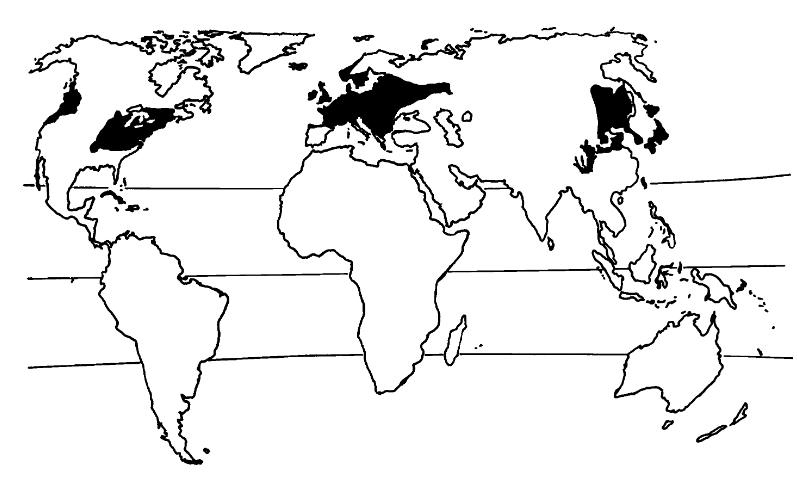
\includegraphics[scale=.5]{DeciduousMap.png}
\caption{Main areas of the temperate forests across the northern hemisphere}
\end{figure}

\subsubsection{Lattitude}

\subsubsection{Countries}

\subsection{Climate}
Climate (rainfall, temp., etc.)


\subsection{Human Interaction}


\subsubsection{Harvesting of Wood}

\subsubsection{Dams for Energy}
Humans use high flowing rivers for energy. While this seems as though it would be an ideal source of healthy energy, the reduced flow can actually be detrimental to 
fish and wildlife in the region. 

Dams can impact water quality, fish life, and cause build up of sediment. 

This sediment builds up oxygen in the water as it decomposes which can cause algae blooms. Algae blooms then cause 
dead zones wherein no oxygen exists. \cite{dd}


 

\subsubsection{Farming on Fertile Soil}
"high population density generally a 
push factor in origin areas (along with land 
scarcity and rural unemployment possibilities), 
but low population density was a pull to the 
frontier. For example, population pressure 
in southern Brazil in the early 1970s was a 
principal factor in spurring colonist farmer 
migration to Rondonia and other frontier states" \cite{population_deforrest}.

\subsubsection{Acid Rain}
"The patchwork of forest has been a boon to research. 
On a tract southwest of the towns (image lower left), the Howland Research Forest is the site of long-term scientific studies supported by NASA, 
the National Science Foundation, the U.S. Forest Service, the U.S. 
Department of Agriculture, and the U.S. Department of Energy. Researchers have observed the effects of acid rain; 
examined the cycling of nutrients through soils; and continually measured how much carbon dioxide the trees absorb, store, and return to the atmosphere. 
The Howland Forest is also a key natural laboratory for observing long-term ecosystem changes" \cite{green_central}

\newpage
\section{Food Web Diagram}

Keystone Species is the deer. 

Detritovores include the woodlouse and fungi or mushroom.

It's not shown in the food web, but the woodlouse and fungi are the final stages in the cycle.

see following page for food web diagram


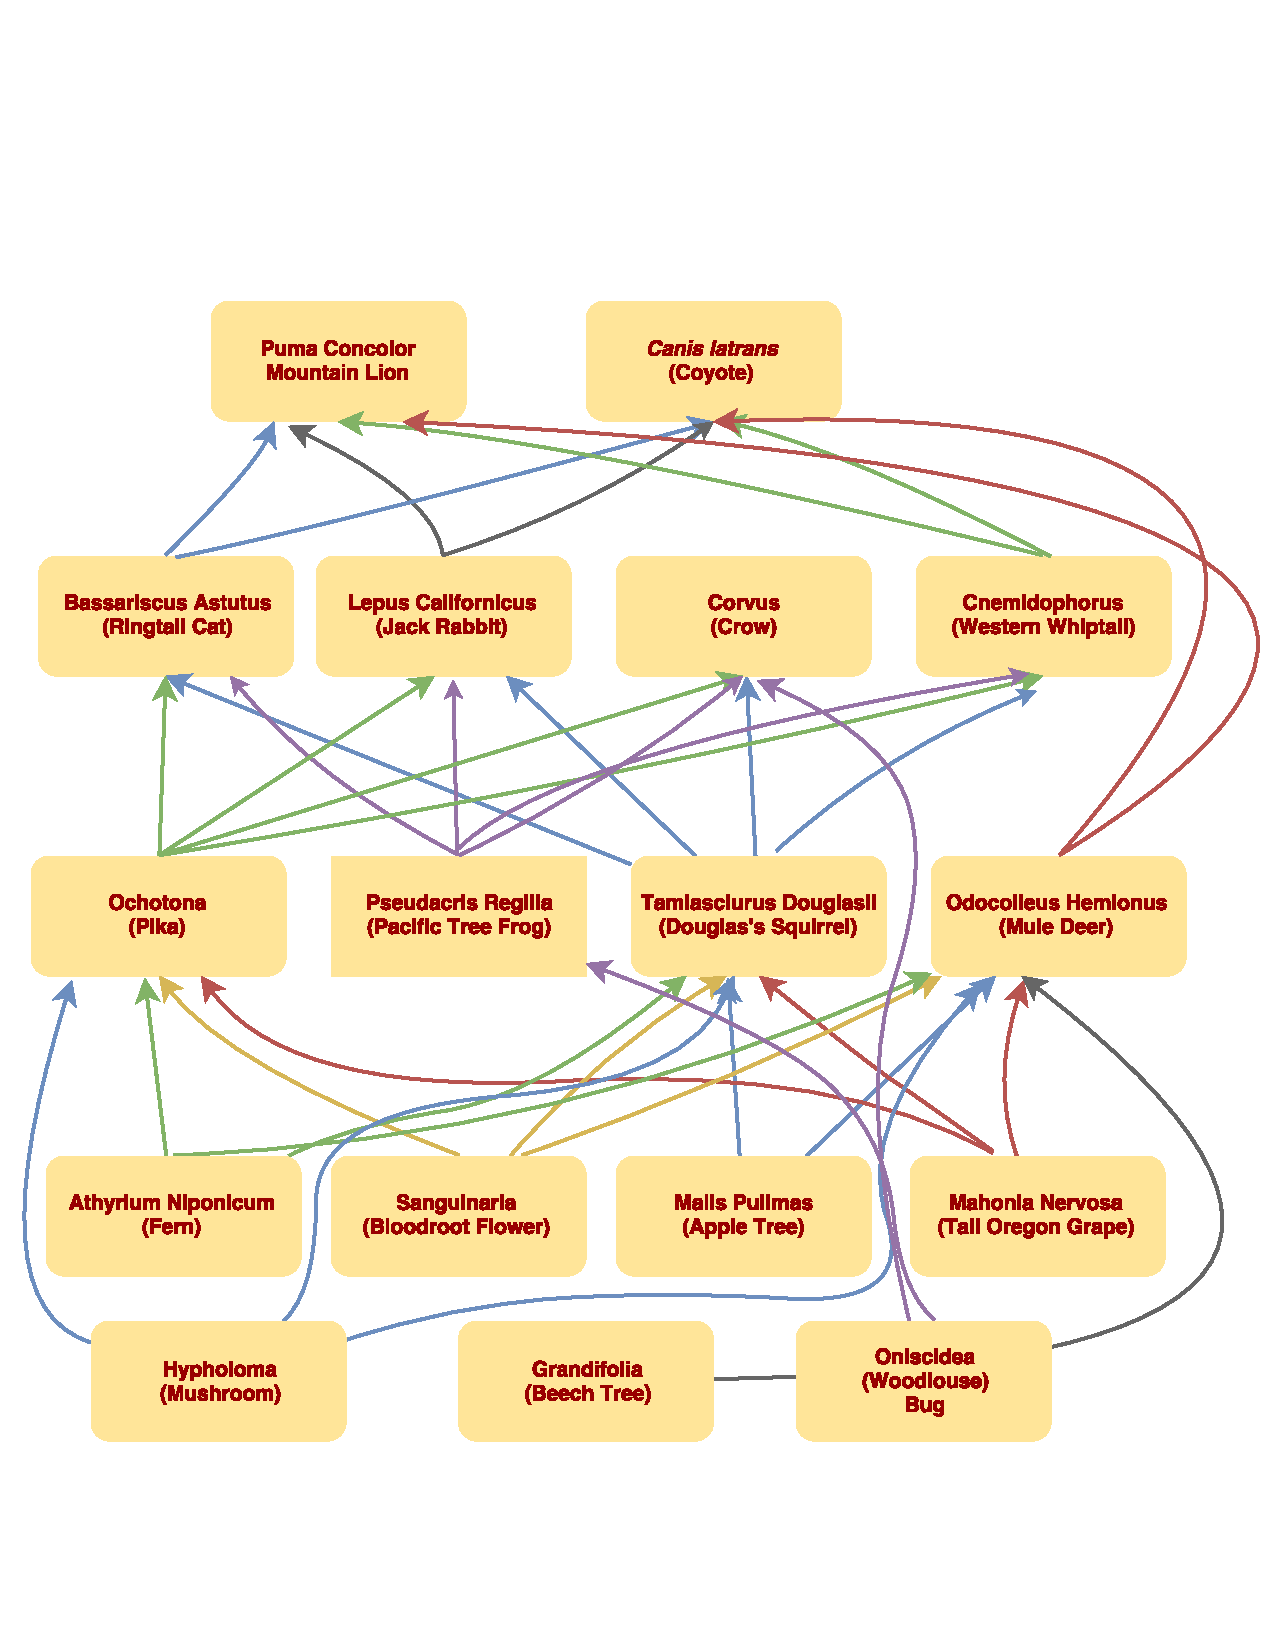
\includepdf{foodweb.pdf}


\section{Niches of Descriptions}


\subsection{Malisa Pulimas or The Apple Tree--Producer}
\subsubsection{Unique Behavioral Adaptations}
The apple itself is an adaptation. The sweetness of an apple entices animals to eat it. In turn, because the seads are not digestible, the seeds will be dispersed by said animal.
The apple tree has also adapted the vascular cambium--a tissue in woody plants that allow it to have a second growth spurt in width. This width is needed to allow the tree to 
carry more nutrients from its roots. \cite{malus}

\subsubsection{Interactions with other species}
The apple tree relies upon bees to help pollinate or reproduce. Bees will collect nectar from one flower, and then unwittingly distribute nectar on another. 

Again, the apple tree also relies upon other animals to distribute its seeds.

\subsubsection{Where Does it Live}
The apple tree can be found in deciduous forests all over the globe, but it's particularly present in Europe and the Eastern United States.





Unique physical or behavioral adaptations that allow it to survive in that biome. (examples - hibernation in bears, thick double fur coat of musk ox, etc.)

Particular interactions with other species (what species does it interact with as predators, prey, herbivores, competitors, symbiotic relationships).

Where does it live? (soil dwelling, tree dwelling, burrow, etc.)

What does it eat? How and where does it search for food?

How does it interact with abiotic factors in the habitat (soil, water, etc?)

Other important relationships within its habitat (include humans if present)


\subsection{Odocoileus Hemionus or Mule Deer--Primary Consumer}
\subsubsection{Unique Behavioral Adaptations}
Mule deer have developed the instinct to flee as they live alongside many predators. The also travel in herds.

\subsubsection{Interactions with other species}
The mule dear are prey for a number of other species, and they also form heads because of this.

\subsubsection{Where Does it Live}
The mule dear lives mostly in the North-Western Americas.

\subsection{Corvus or The Crow--Secondary Consumer}
\subsubsection{Unique Behavioral Adaptations}
The crow is an extremely smart bird. It is also able to eat a variety of foods as an omnivore. 
They have adapted teamwork and even stand guard for others during feeding time.

\subsubsection{Interactions with other species}
The crow is at the top of it's food web in that it will eat nearly anything, but nothing really eats it.

One species the crow has a history of interaction with is us humans! In fact at times crows have been considered a pest as they
can damage crops. In some parts of the world, crows are controlled through forms of hunting, trapping, poison, and or scare tactics.


\subsubsection{Where Does it Live}
Crows can live in forests and near humans. Geographically they are found in deciduous environments all over the world.


\subsection{Canis Iatrans or The Coyote--Predator}
\subsubsection{Unique Behavioral Adaptations}


\subsubsection{Interactions with other species}
The coyote will eat anything from mice to deer. As such, it interacts with its prey. 

Beyond this, humans have controlled and hunted coyotes throughout history. At one point
they were hunted for their furs.  

Coyotes don't often attach humans, but it does happen. Mostly coyotes will harm livestock and 
are controlled to prevent this.

\subsubsection{Where Does it Live}
The coyote lives throughout almost all of North America. Coyotes tend to sleep in a communal den to 
stay warm.

\subsection{Oniscidea or Woodlouse--detritavore}
\subsubsection{Unique Behavioral Adaptations}
The woodlouse's color helps it to blend in. It has also developed a hard shell, and can curl up into 
a ball for protection from predators.

\subsubsection{Interactions with other species}
When the woodlouse and the earthworm are both consuming cellulose or wood, it has been found that the
rate of consumption is greater than it would have been separately. This indicates a sort of 
symbiotic relationship. \cite{woodlice}

\subsubsection{Where Does it Live}
The wood louse lives in dark damp places such as under rocks and trees. The woodlouse can be found in 
 temperate regions throughout the world.

\bibliography{Biome}


\end{document}  
